%!TEX root = ../../super_main.tex

\section{The Campaign Model}

A \emph{snapshot} is conceptually a time snippet of the reality around a participant. The information in a \emph{snapshot} consists of sensor readings of the devices of the participant, and some \emph{label} that is derived by explicitly asking the participant. 

This campaign desires to get readings from a heartbeat sensor, an accelerometer and a GPS and ask questions regarding alcohol.

\begin{figure}[!htbp]
    \centering
    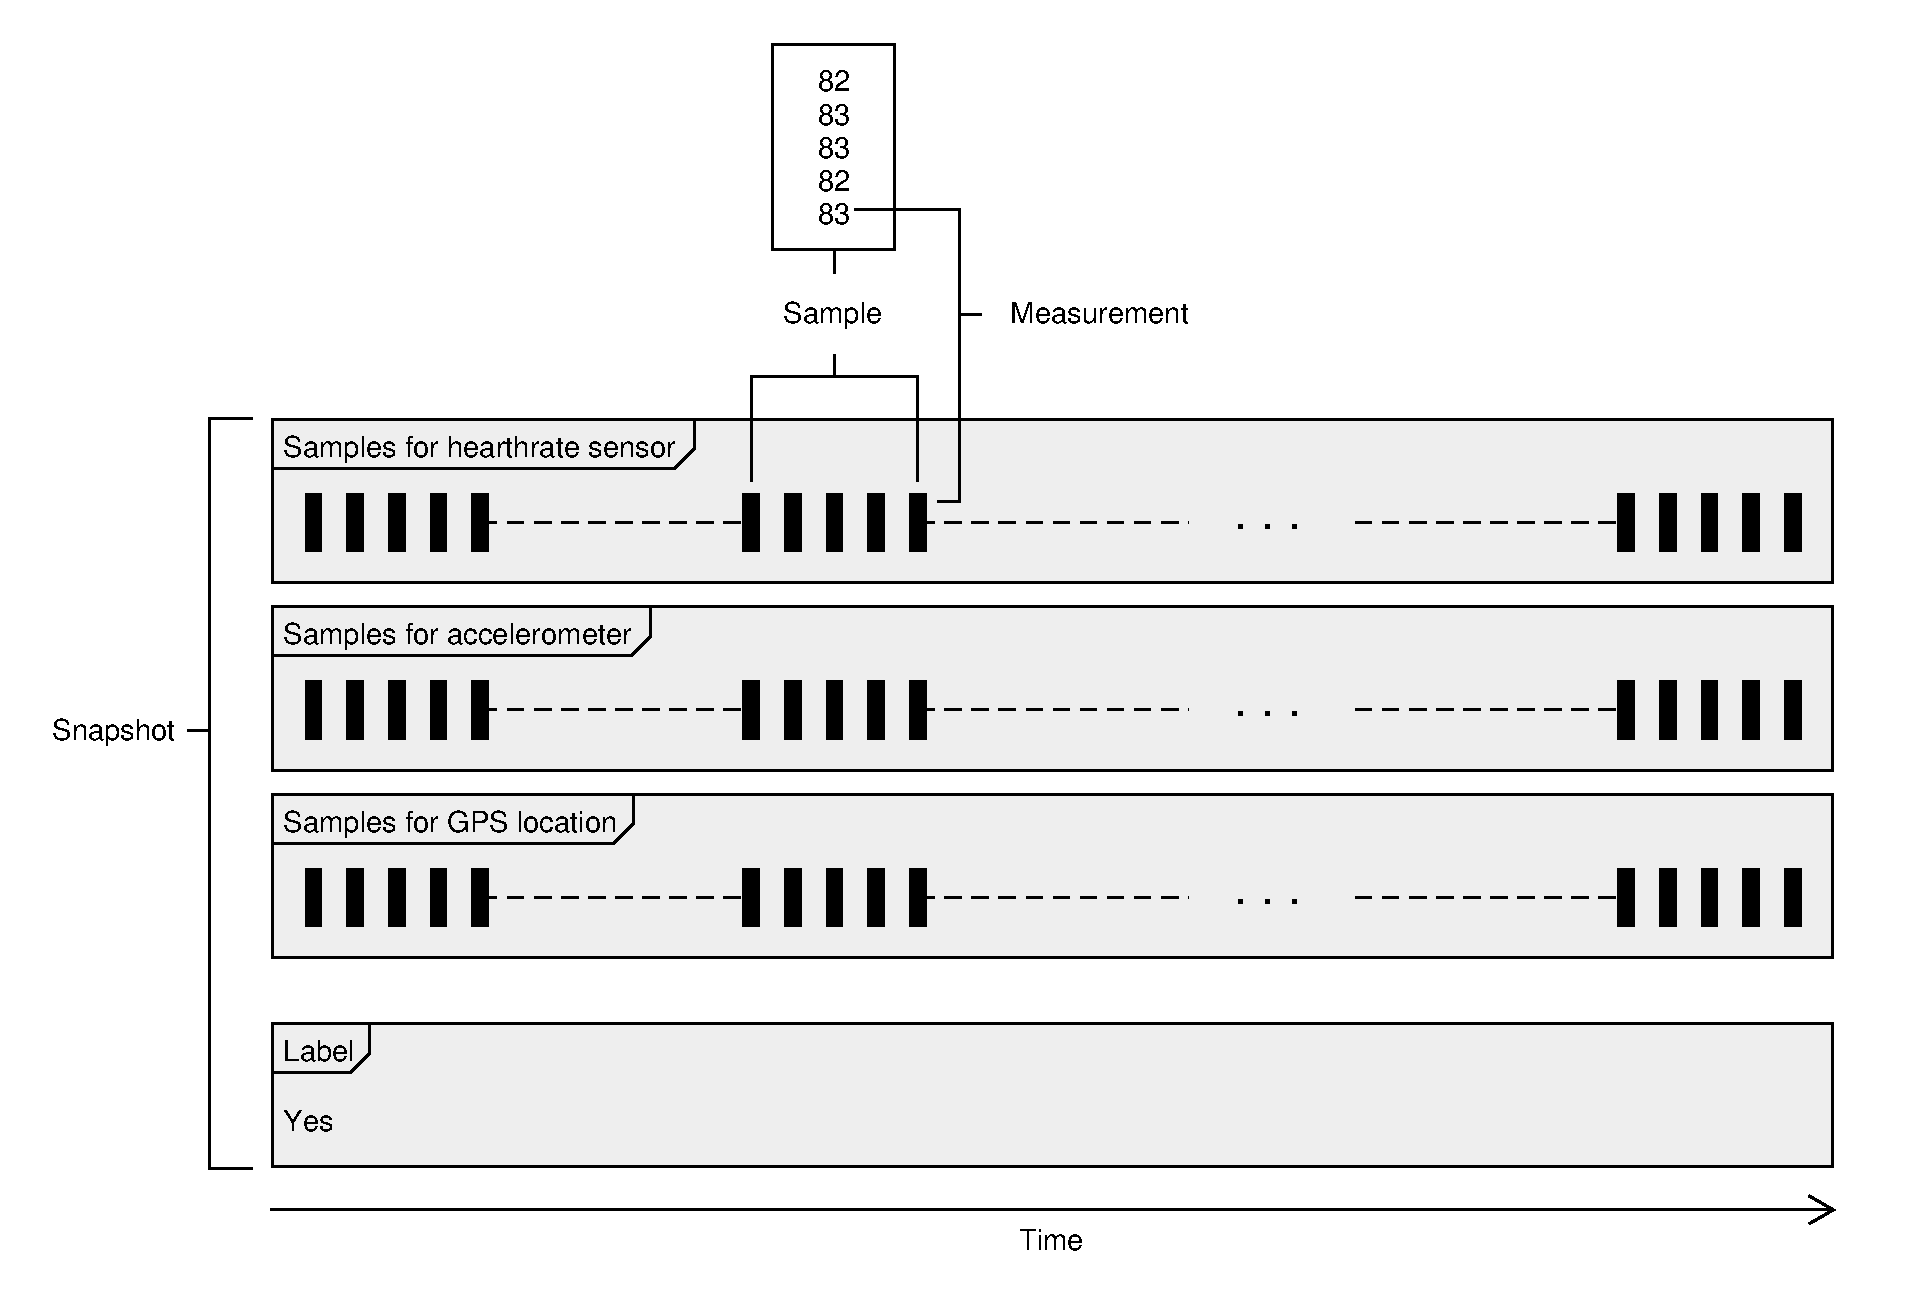
\includegraphics[width=\textwidth]{gathering_sensor_data/snapshot}
    \caption{Snapshot.}
    \label{fig:snapshot_example}
\end{figure}
\FloatBarrier

An example of such a snapshot could be as seen in \figref{fig:snapshot_example}. This have outputs from the sensors specified in the campaign. These measurements have some special temporal structure which will be described REF-TIL-TEMPORALITY. Besides sensor readings a \emph{snapshot} also have a \emph{label} associated. 





\todo[inline]{Beskriv hvad en campaign er i koden, brug gerne klassediagrammet til at forklare det!}

\begin{figure}[!htbp]
    \centering
    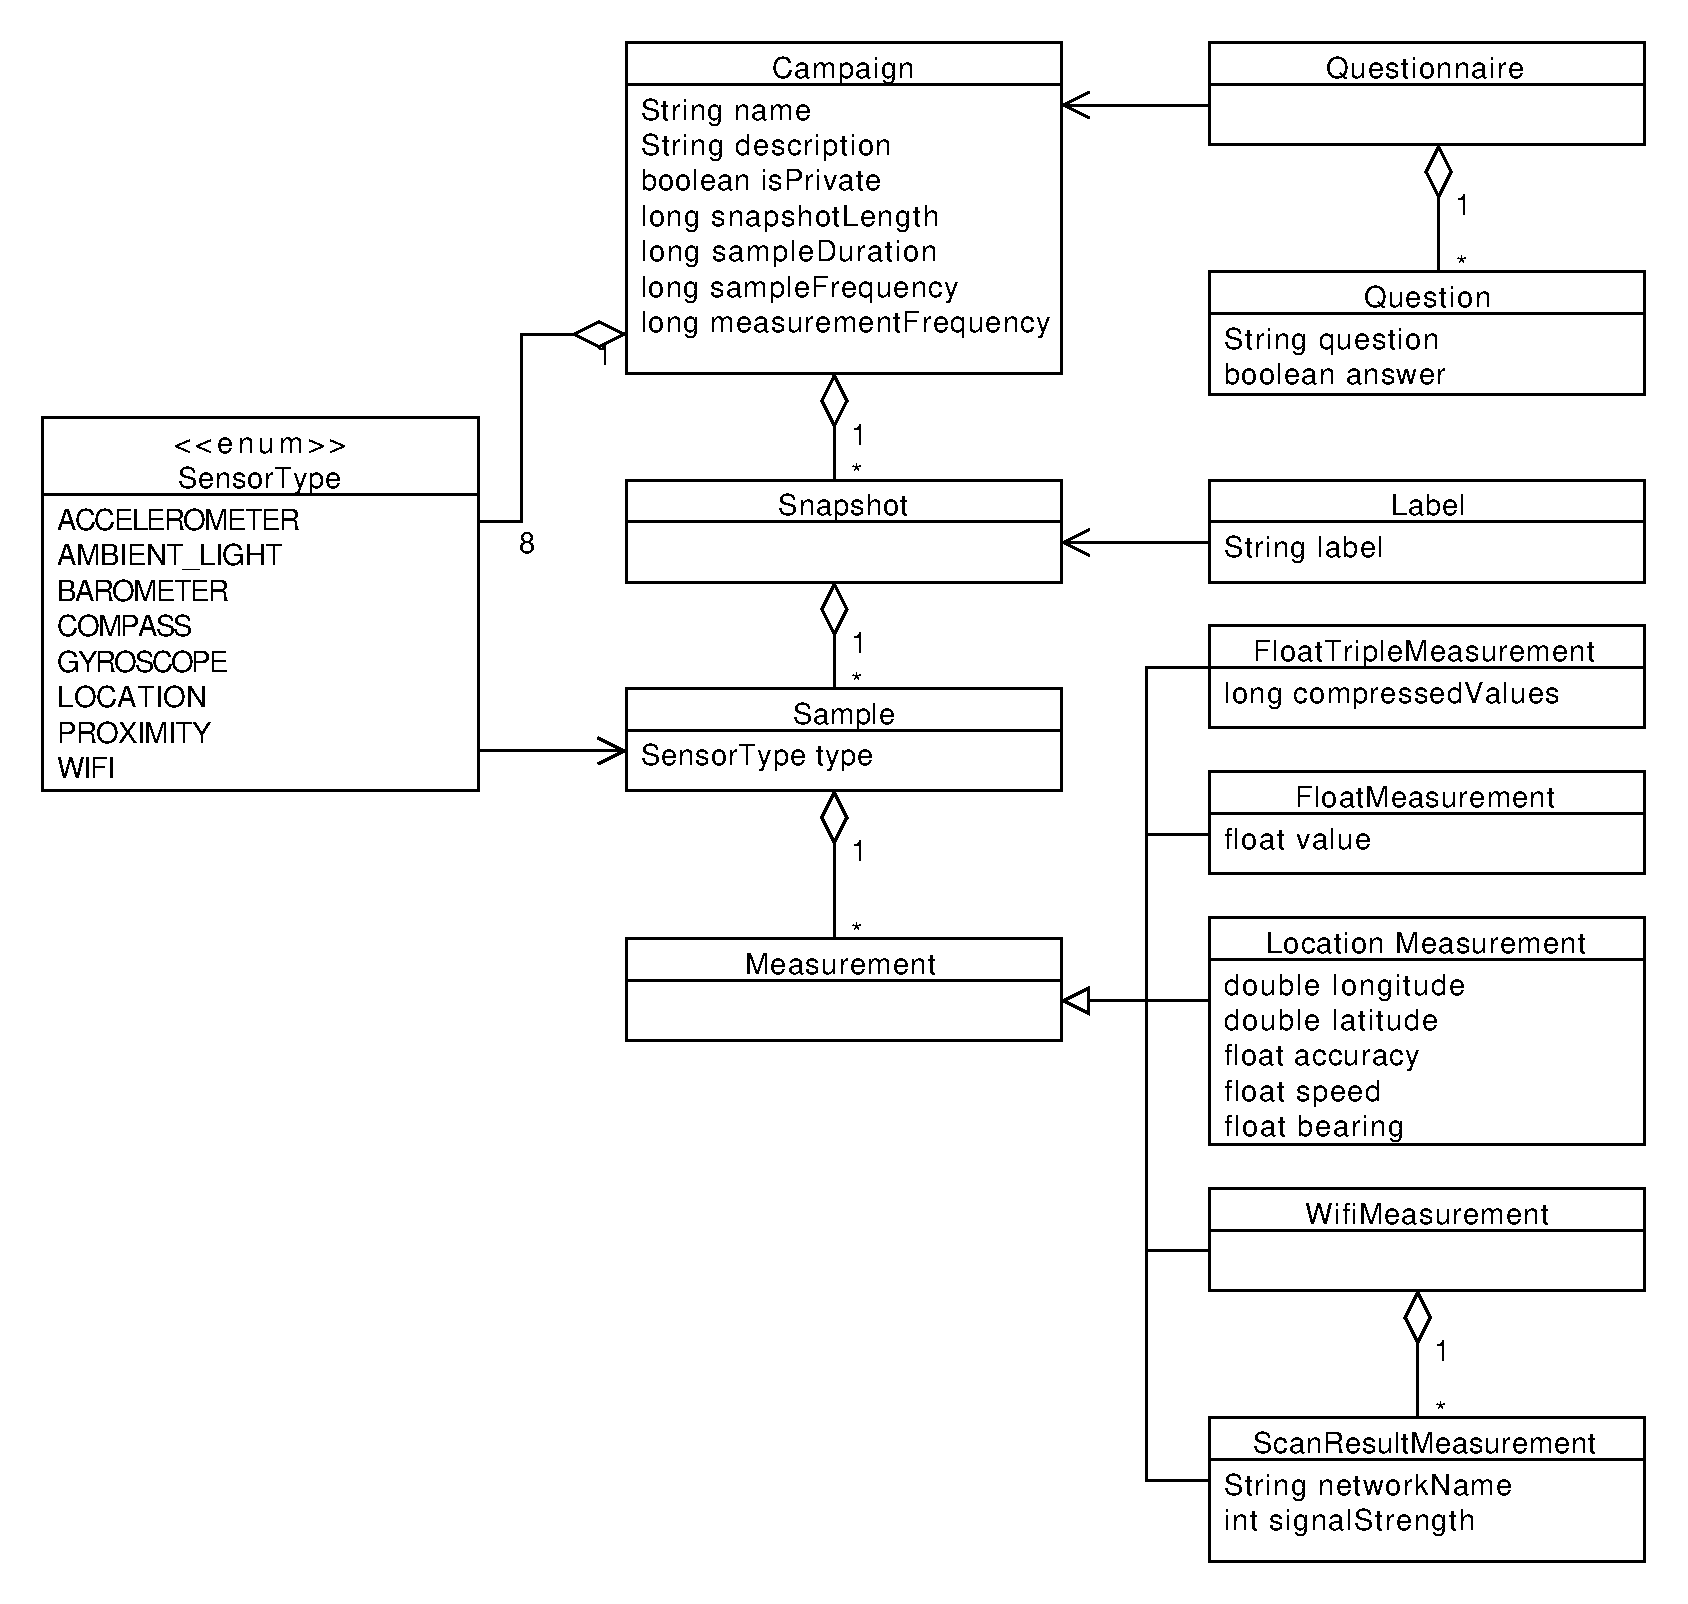
\includegraphics[width=\textwidth]{graphic/gathering_sensor_data/model_class_diagram.pdf}
    \caption{Class Diagram of the campaign model.}
    \label{fig:model_class_diagram}
\end{figure}
\FloatBarrier

\todo[inline]{ref til figur}

\subsection{Questionnaires}
We had come to the conclusion that customers should be able to define questionnaires to be a part of the data collection \secref{sec:human_activity_recognition}. Customers should be able to define one or more separate questions or more generally data inputs which combined should make out a questionnaire model. 
\\\\
Simple boolean yes/no questions can directly be combined to create a discrete amount of labels or classes which can later be used as targets for an AI model but more open inputs, which for instance can be used for regression or as more diverse features, should also be possible. \todo{Overvej om vi når at implementere continuous inputs}
\\\\
A questionnaire specification should be transformable to a format which can be easily be parsed and send from the server to the collecting devices. We have therefore implemented a questionnaire to be Java Parcelable. \todo{Overvej at ændre det her hvis vi gør det til JSON ting i stedet}

